\documentclass[12pt,a4paper]{article}
\usepackage[T1]{fontenc}
\usepackage{natbib}
\usepackage{graphicx}
\usepackage{pdflscape}
\usepackage{amsmath}
\renewcommand{\figurename}{Şekil}
\renewcommand{\refname}{Kaynakça}
\date{}
\title{TensorFlow ile Meyve Veri Seti Üzerinde Eğitilmiş Bir Nesne Tanıma Modelinin C++'a Aktarılması ve Tespitin Gerçekleştirilmesi}
\author{Baranalp Öztürk}

\begin{document}
	\begin{figure}
		\centering
		
\includegraphics{ksbu.jpg}
	\end{figure}
	\maketitle
	\maketitle
	\begin{center}
	\section*{Giriş}
	\end{center}
Bu projede, kavun, çilek, ananas, portakal, mango, kivi, kiraz, avokado, muz ve elma gibi on farklı meyve türünün verileri toplanarak bir yapay zeka modeli geliştirilecektir. Python kullanılarak TensorFlow kütüphanesi ile bir derin öğrenme modeli oluşturulacak ve meyve görüntüleri üzerinde eğitilecektir. Model, farklı meyve türlerini tanımak için optimize edilecek, performansı değerlendirilecek ve gerekli iyileştirmeler yapılacaktır. Eğitim tamamlandıktan sonra, model C++ programlama dili kullanılarak export edilecek ve algılama işlemleri için entegre edilecektir. Bu, meyve türlerini tanımlamak için bir görüntü işleme uygulaması oluşturulmasını sağlayacaktır. Projede ayrıca Roboflow'un otomatik etiketleme özelliği kullanılarak intersection over union (IoU) değerlerinin değerlendirilecektir. Bu özellik, etiketleme sürecini hızlandırarak ve insan hatalarını azaltarak IoU değerlerinin doğruluğunu artırabilir. Bu yöntem, projenin başarısını değerlendirmek ve geliştirmek için önemli bir araç olacaktır.
	\begin{enumerate}
		\clearpage
		\item		
		
		
		\begin{center}
			\section*{Literatür Araştırması}			
		\end{center}		
		
		Mantarların Türk ve Dünya mutfaklarında kullanımı hızla artmakta, özellikle son
		yıllarda yabani mantar toplayıcılığı ve tüketiminde önemli artışlar yaşanmaktadır.
		Çevremizde sıkça gözlemlediğimiz gıda zehirlenmelerinin birçoğunu mantar zehirlenmeleri oluşturmaktadır. Öyle ki bu oran erişkinlerde mantar zehirlenmeleri tüm
		akut zehirlenme vakalarının yaklaşık yüzde 7'sini oluşturmaktadır. Ülkemizin kırsal kesimleri
		başta olmak üzere pek çok yerinde halk mantarları toplayarak gıda olarak tüketmektedir.
		Ülkemizde yeterli bilgiye sahip olmayan kişiler tarafından toplanan mantarların besin
		olarak tüketilmesi ile zehirlenmeler ve ne yazık ki ölümler görülebilmektedir. Bu
		çalışmada doğada kolaylıkla yetişebilen mantarların insanlar üzerindeki olumsuz
		etkilerini azaltmak amacıyla, insanların mantar kullanımında bilgi sahibi olmalarını
		sağlayarak bilinç düzeylerini artırmak için derin öğrenme tabanlı mobil uygulama
		tasarlanmıştır. Çalışmada ayrıca açık kaynak kod olarak sunulan, Google ve bağımsız
		geliştiriciler tarafından geliştirilen Tensorflow ve Keras kütüphaneleri kullanılmıştır.
		Android Studio ve Java programlama dili kullanılarak tasarlanan mobil uygulamaya derin
		öğrenme metotlarından VGG16 entegre edilerek kameradan görüntüsü alınan mantar
		tespit edilerek kullanıcıya özellikleri sunulmaktadır. Araştırma bulgularına uygulanan
		istatistiksel analizler sonucunda doğruluk oranı yüzde 81.75 olarak hesaplanmıştır
		\cite{akin2023dogada}.
		
		
		
		
		
		
		
		
		
		Meyve, Endonezya'da oldukça potansiyelli bir üründür. Hasat sırasında meyve üretimi oldukça bol olsa da, yavaş hasat süreci kaliteyi azaltır. Sonuç olarak, satış fiyatı düşüktür. Araştırmamızda, çoklu meyveleri sınıflandırmak için daha hızlı R-CNN kullanarak Derin Öğrenme yöntemi öneriyoruz. Kullanılan girişler mango ve pitaya meyveleridir. Veri kümesi, hasat zamanında bir çiftçiden alınan gerçek verilerden oluşur ve daha sonra eğitim nesne tespiti için mango ve pitaya olmak üzere 2 sınıfa ayrılır. TensorFlow platformunda MobileNet modelini kullandık. Bu çalışmada, yaklaşık yüzde 99'luk bir doğruluk skoru elde ettik. Bu yöntem, meyve kalitesini korumak için gerçek zamanlı olarak çoklu meyvelerin sıralama işlemini geliştirmek için oldukça uygundur \cite{8628566}.
		
		
		
		
		
		\clearpage
		
		
		Son yıllarda, nesne tespiti ve Desen Analizi alanında kapsamlı bir çalışma yapma konusunda büyük bir büyüme yaşanmaktadır. Sistemimizde, nesne tanıma ve desen analizi alanında makine öğrenimi ve derin öğrenme yaklaşımına dayalı bir tespit yöntemi üzerinde iyileştirmeler ve deneyler yaptık. Nesne tespitini, sınıf olasılıklarını ve sınırlayıcı kutuları mekansal olarak ayrılmış karşılık gelen bir gerileme sorunu olarak varsayıyoruz. Nesne tespiti, Desen Analizi ve izleme için birçok önde gelen algoritma tasarlanmıştır, bu da kenar izleme, renk bölütleme ve desen eşleştirmeyi içerir. Tek bir sinir ağı, bir döngüde tam görüntüden sınıf olasılıklarını ve sınırlayıcı kutuları doğrudan tahmin edebilir. Bu nedenle, Tensorflow'un yardımıyla video analizi yapmak için çeşitli sinir ağı algoritmalarını, YOLOv3, Tek Atışlı Çoklu tespit algoritmasını kullanıyoruz. Çerçeve, nesneleri sürekli olarak algılayacak ve kameradan algılanan girişlerden gerektiğinde kareler yakalayıp nesneyi tahmin etmek ve deseni eşleştirmek için kullanılabilir. Gerçek zamanlı video işleme ve tek bir kamera kullanılarak başarıyla tamamlanmıştır. Önerilen sistem, karmaşık, gerçek zamanlı, düz olmayan ortamlarda işlem yapabilecek esnek bir yapıya sahiptir\cite{9076486}.			
		\\*				
		Tabakalar ve dikkat mekanizmalarını derinleştirerek, küçük hedef kusurlarını tanıma yeteneğini artıran, arka plan gürültüsünü azaltan ve hesaplama verimliliğini artırmak için orijinal evrişim modüllerini derinlikli ayrılabilir evrişim ile değiştiren, hafif bir seramik karo tespit sistemi olan geliştirilmiş YOLOv5s modeline dayanan bir tespit yöntemi öneriyoruz. Deney sonuçları, modelimizin küçük kusurlar ve yetersiz özellik bilgisi ile ilgili sorunları etkili bir şekilde ele aldığını ve tespit doğruluğunu artırdığını göstermektedir					
		\cite{WAN202211085}.\pagebreak
		
\begin{figure}[h]
	\centering
	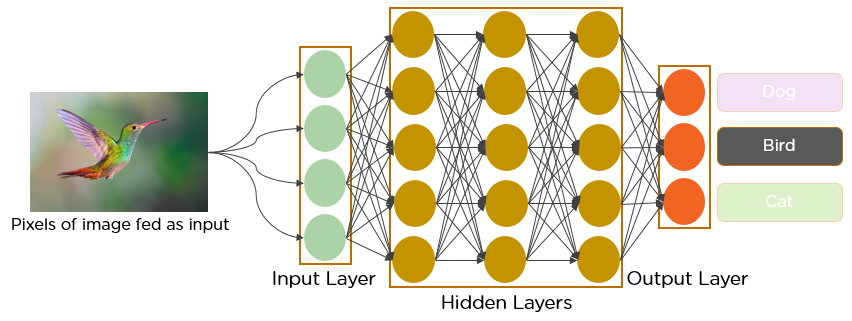
\includegraphics[width=\textwidth]{bird.png}
	\caption{CNN Model}
	\label{fig:grafik}
\end{figure}
		
\begin{figure}[h]
	\centering
	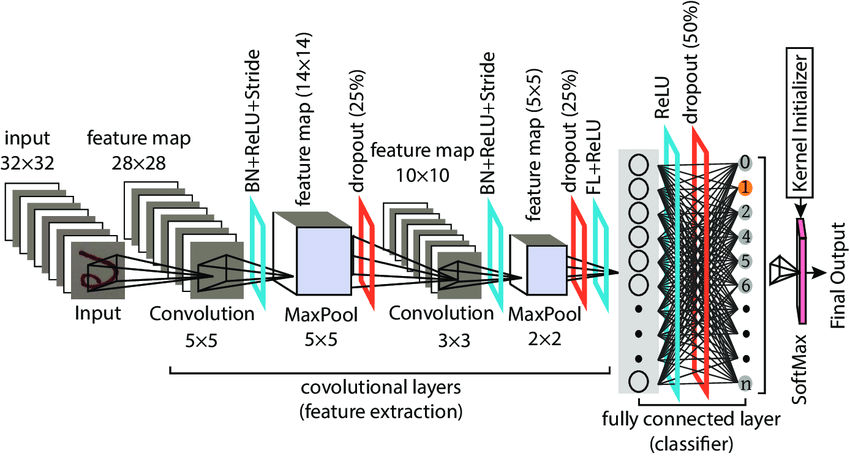
\includegraphics[width=\textwidth]{model.png}
	\caption{CNN Model}
	\label{fig:grafik}
\end{figure}

				
				
					\begin{figure}[h]
						
						\centering
					
						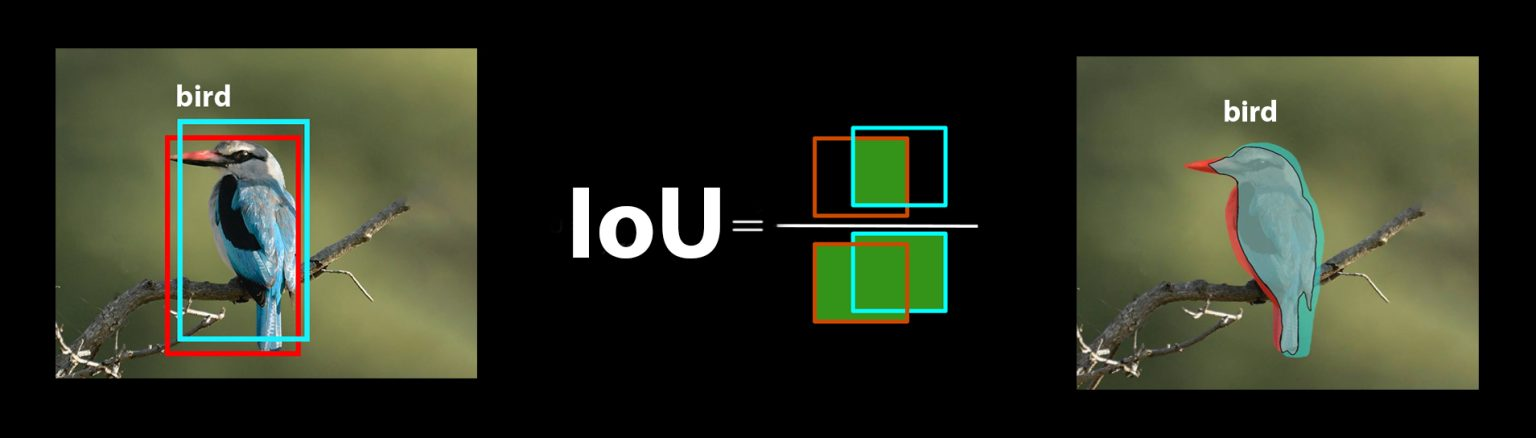
\includegraphics[width=1.1\textwidth, height=0.8\textheight]{union.jpg}
						
						
					\[
				\text{IoU} = \frac{\text{Birleşim Alanı}}{\text{Kesişim Alanı}} = \frac{60}{100 + 80 - 60} = \frac{60}{120} = 0.5
				\]
					
						\caption{Instruction Over Union}
						\label{fig:grafik}
					\end{figure}
				
				
	\end{enumerate}
	\begin{center}
	\pagebreak
		\section*{Metodoloji}
		\begin{enumerate}
			\item Modelin Export Edilmesi: Eğitilmiş TensorFlow modelinin C++ tarafında kullanılabilmesi için öncelikle modelin uygun bir formatta export edilmesi gerekir. TensorFlow, SavedModel veya FrozenGraph formatlarını destekler. Bu formatlardan birini seçerek modelinizi export etmelisiniz.
			\item TensorFlow C++ API'nin Kullanılması: TensorFlow C++ API, eğitilmiş modelin yüklenmesi ve görüntü işleme işlemlerinin gerçekleştirilmesi için kullanılır. API, modeli yüklemek, görüntü verilerini hazırlamak, tahmin yapmak ve sonuçları işlemek için gerekli olan fonksiyonları sağlar.
			\item 	Görüntü Verisinin Hazırlanması: Görüntü işleme işlemlerini gerçekleştirebilmek için girdi görüntülerin uygun formatta hazırlanması gerekir. Bu adımda, görüntülerin okunması, ön işleme adımlarının uygulanması ve TensorFlow tarafından kullanılabilen bir veri yapısına dönüştürülmesi gerekebilir.
			\item  Tahmin Yapma İşlemi: TensorFlow C++ API kullanılarak eğitilmiş model üzerinde tahmin yapılır. Girdi olarak hazırlanan görüntüler modelin girdisi olarak kullanılır ve modelden tahminler elde edilir.
			\begin{enumerate}
				\section*{TensorFlow C++ API Neleri İçerir}
				\item Graph Loading (Graf Yükleme): TensorFlow C++ API, eğitilmiş bir TensorFlow modelinin grafını (graph) yüklemek için fonksiyonlar sağlar. Bu, önceden eğitilmiş bir modelin mimarisini ve ağırlıklarını yüklemeyi mümkün kılar.
				\item Session Management (Oturum Yönetimi): API, TensorFlow modeliyle etkileşimde bulunmak için oturum (session) yönetimi sağlar. Bu, modelin belirli bir giriş verisine göre çıktıları tahmin etmek için oturum oluşturmayı ve sonlandırmayı içerir.
				\item Input Data Handling (Giriş Verisi İşleme): API, modelin giriş verilerini hazırlamak ve işlemek için gerekli fonksiyonları sağlar. Bu, giriş verilerini modelin beklediği formata dönüştürmeyi ve uygun şekilde işlemeyi içerir.
				\item Inference (Tahmin): API, yüklenen TensorFlow modelini kullanarak tahmin yapmak için fonksiyonlar sağlar. Bu, modelin giriş verisine dayalı olarak çıktıları tahmin etmeyi içerir.
				
				\pagebreak
				\begin{center}
					\section*{Veriler}
				\end{center}
				
				
				
				Bu çalışmada, toplamda 35MB boyutunda 10 farklı meyve türünün resimlerini içeren bir veri kümesi kullanılmıştır. Bu meyve türleri ve resim sayıları şu şekildedir:
				
				\begin{itemize}
					\item Watermelon: 315 adet
					\item Strawberries: 309 adet
					\item Pineapple: 320 adet
					\item Orange: 297 adet
					\item Mango: 320 adet
					\item Kiwi: 320 adet
					\item Cherry: 319 adet
					\item Banana: 318 adet
					\item Avocado: 315 adet
					\item Apple: 267 adet
				\end{itemize}
				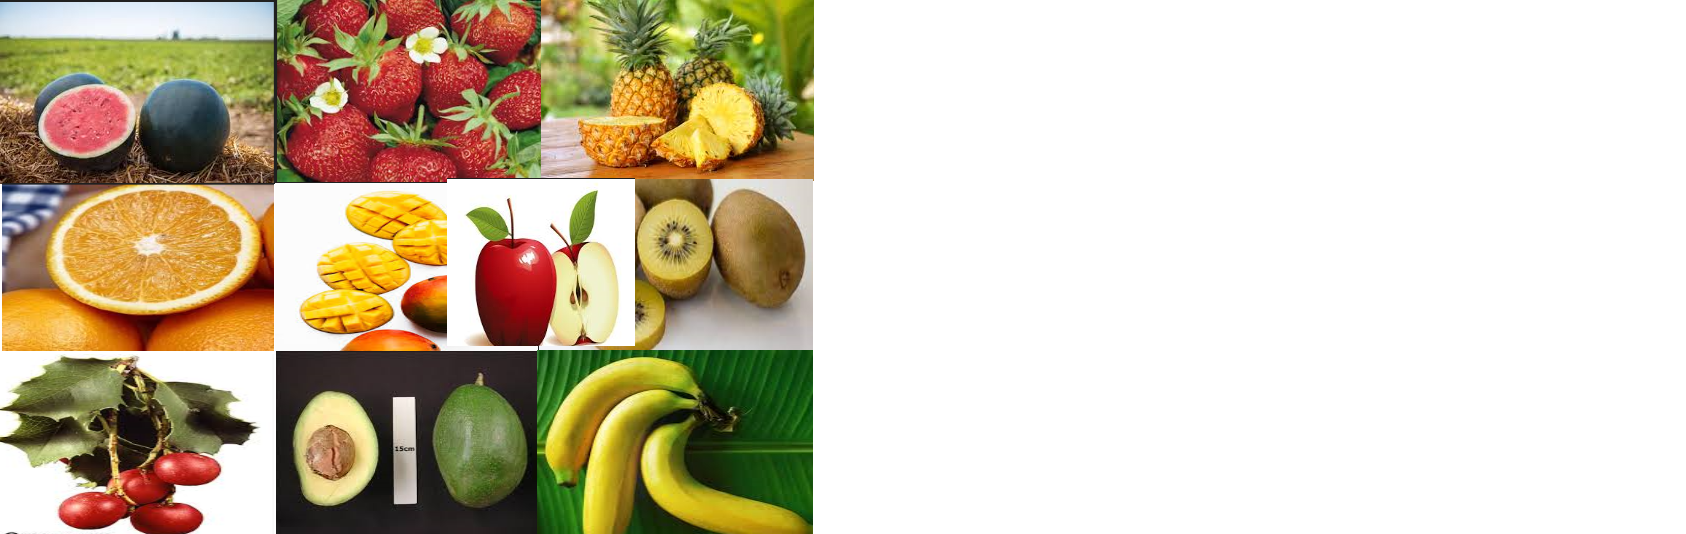
\includegraphics[scale=0.4]{train.png}
				
				Her bir resim, 200x200 piksel boyutunda ve JPEG formatında kaydedilmiştir. Bu resimler, derin öğrenme modelinin eğitilmesi ve test edilmesi için kullanılmıştır.		
				Bu veri kümesi, farklı meyve türlerinin doğru bir şekilde tanınması ve sınıflandırılması için geliştirilen yapay zeka modellerinin eğitiminde kullanılan temel veri kaynağıdır. Veri seti, meyve türlerini çeşitli açılardan ve ortamlardan içeren çeşitli görüntülerle zenginleştirilmiştir.Bu projenin başarılı olması durumunda, yapay zeka destekli robotlarla yapılan tarım alanında önemli gelişmeler sağlanabilir. Yapay zeka ve görüntü işleme tekniklerinin kullanımıyla donatılan tarım robotları, tarım verimliliğini artırmak, iş gücünden tasarruf etmek ve tarım süreçlerini otomatikleştirmek için etkili bir araç olabilirler. Bu robotlar, çeşitli meyve türlerini tanımlayıp algılayarak, hasat sürecini optimize edebilir, hastalıklı veya olgunlaşmış meyveleri tespit edebilir.  
				
				
				\clearpage
				
				\begin{center}
					\section*{Beklenen Sonuçlar}
				\end{center}
				Bu projenin başarılı olması durumunda, yapay zeka modelinin geliştirilmesi ve uygulanmasıyla çeşitli meyve türlerinin doğru bir şekilde tanınması ve algılanması mümkün olacaktır. Beklenen sonuçlar arasında, TensorFlow kullanılarak eğitilen derin öğrenme modelinin on farklı meyve türünü doğru bir şekilde tanımlayıp algılayabilmesi ve \%97 tespit yüzdesi beklenir. C++ programlama dili kullanılarak bu modelin export edilip entegre edilmesi, ve Roboflow'un otomatik etiketleme özelliği kullanılarak IoU değerlerinin artırılması ve modelin doğruluğunun iyileştirilmesi yer almaktadır. Projenin başarılı olması durumunda, geliştirilen görüntü işleme uygulamasının meyve türlerini tanımlama ve algılamada yüksek doğruluk sağlayacağı öngörülmektedir. Bu sonuçlar, meyve tanıma ve algılama konusundaki yapay zeka teknolojisinin gelişimine ve tarım endüstrisindeki verimliliğin artmasına önemli bir katkı sağlayacaktır.				
				Ayrıca, projenin başarılı olması durumunda, yapay zeka destekli robotlarla yapılan tarım alanında da önemli gelişmeler sağlanabilir. Bu ilerlemeler, tarım endüstrisinde verimliliği artırabilir, iş gücü maliyetlerini azaltabilir ve tarım ürünlerinin kalitesini ve miktarını artırabilir. Ayrıca, çevresel etkileri azaltarak sürdürülebilir tarım uygulamalarının yaygınlaşmasına da katkıda bulunabilir. Bu nedenle, projenin başarılı olması, yapay zeka destekli robotların tarım alanında kullanımının yaygınlaşmasına ve tarımın gelecekteki sürdürülebilirliğine önemli bir katkı sağlayabilir.
				
					\begin{figure}[h]
						
						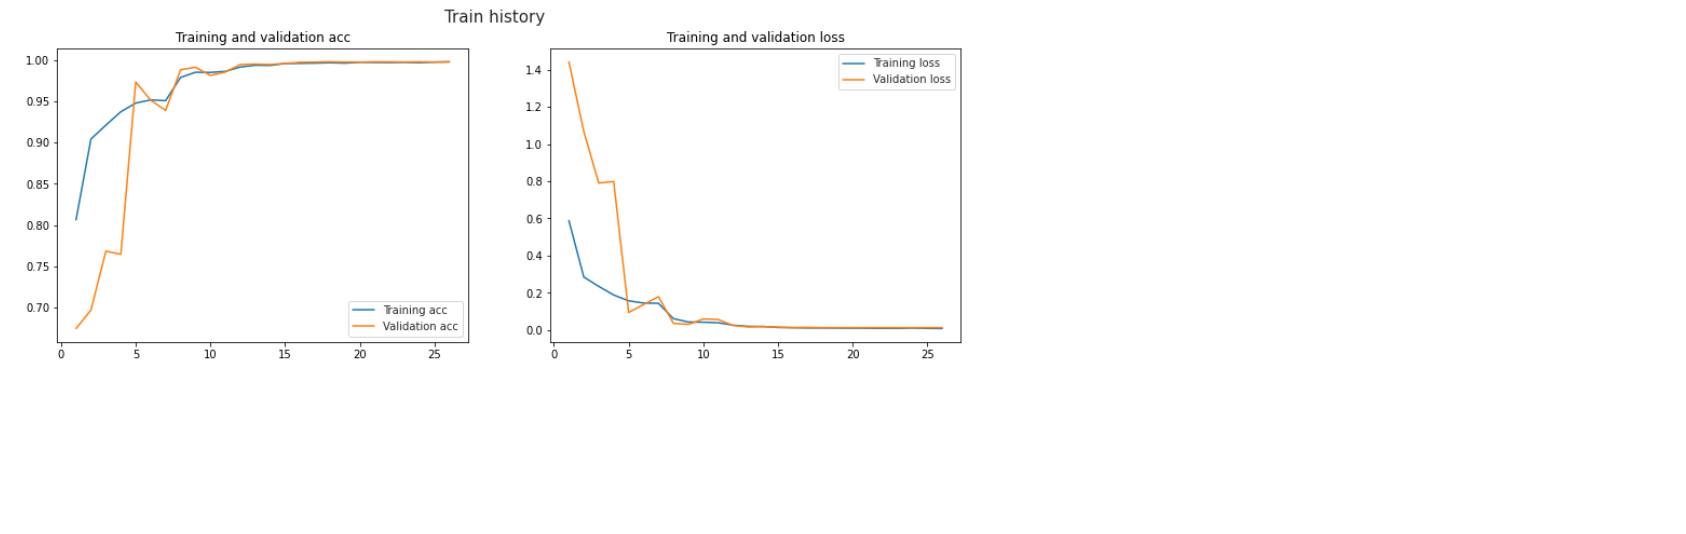
\includegraphics[width=1.4\textwidth]{expectation.png}
					
					\caption{Beklenen Başarı Sonuçları}
					\label{fig:grafik}
					\end{figure}
				
				
				
				
					\begin{landscape}
					\begin{figure}
						
						\centering
						\section*{Gant Şeması}
						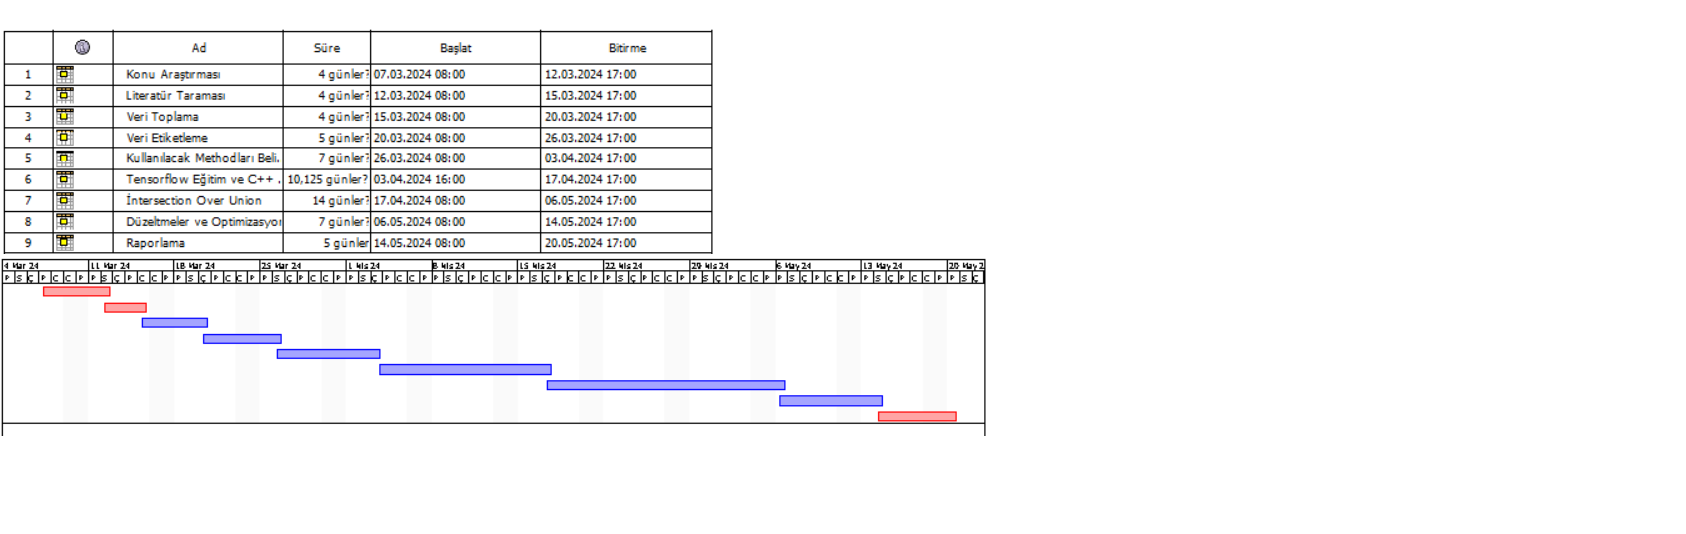
\includegraphics{gant.png}
						
						\label{fig:gant}
					\end{figure}
				\end{landscape}
				
				
				
				
			\end{enumerate}
		\end{enumerate}
		
	
			
		
		
		
		
		
		
	\end{center}
	\bibliographystyle{plain}
	\bibliography{references}
	
	
\end{document}